%%%%%%%%%%%%%%%%%%%%%%%%%%%%%%%%%%%%%%%%%%%%%%%%%%%%%%%%%%%%%%%%%%%%%%%%%%%%
% AGUJournalTemplate.tex: this template file is for articles formatted with LaTeX
%
% This file includes commands and instructions
% given in the order necessary to produce a final output that will
% satisfy AGU requirements, including customized APA reference formatting.
%
% You may copy this file and give it your
% article name, and enter your text.
%
% guidelines and troubleshooting are here: 

%% To submit your paper:
\documentclass[final]{agujournal2019}
\usepackage{url} %this package should fix any errors with URLs in refs.
\usepackage{lineno}
\usepackage[inline]{trackchanges} %for better track changes. finalnew option will compile document with changes incorporated.
\usepackage{soul}
%\linenumbers
\usepackage{microtype}
\usepackage{lmodern}
\usepackage{changepage}

\renewcommand{\thefigure}{S\arabic{figure}}
\renewcommand{\thetable}{S\arabic{table}}
%%%%%%%
% As of 2018 we recommend use of the TrackChanges package to mark revisions.
% The trackchanges package adds five new LaTeX commands:
%
%  \note[editor]{The note}
%  \annote[editor]{Text to annotate}{The note}
%  \add[editor]{Text to add}
%  \remove[editor]{Text to remove}
%  \change[editor]{Text to remove}{Text to add}
%
% complete documentation is here: http://trackchanges.sourceforge.net/
%%%%%%%

\draftfalse

%% Enter journal name below.
%% Choose from this list of Journals:
%
% JGR: Atmospheres
% JGR: Biogeosciences
% JGR: Earth Surface
% JGR: Oceans
% JGR: Planets
% JGR: Solid Earth
% JGR: Space Physics
% Global Biogeochemical Cycles
% Geophysical Research Letters
% Paleoceanography and Paleoclimatology
% Radio Science
% Reviews of Geophysics
% Tectonics
% Space Weather
% Water Resources Research
% Geochemistry, Geophysics, Geosystems
% Journal of Advances in Modeling Earth Systems (JAMES)
% Earth's Future
% Earth and Space Science
% Geohealth
%
% ie, \journalname{Water Resources Research}

\journalname{Earth's Future}


\begin{document}

%%%%%%%%%%%%%%%%%%%%%%%%%%%%%%%%%%%%%%%%%%%%%%%
%  TITLE
%
% (A title should be specific, informative, and brief. Use
% abbreviations only if they are defined in the abstract. Titles that
% start with general keywords then specific terms are optimized in
% searches)
%
%%%%%%%%%%%%%%%%%%%%%%%%%%%%%%%%%%%%%%%%%%%%%%%

% Example: \title{This is a test title}

\title{Supporting Information for: ``Intensifying renewable energy droughts in the Western U.S. amid evolving infrastructure and climate``}

%%%%%%%%%%%%%%%%%%%%%%%%%%%%%%%%%%%%%%%%%%%%%%%
%
%  AUTHORS AND AFFILIATIONS
%
%%%%%%%%%%%%%%%%%%%%%%%%%%%%%%%%%%%%%%%%%%%%%%%

% Authors are individuals who have significantly contributed to the
% research and preparation of the article. Group authors are allowed, if
% each author in the group is separately identified in an appendix.)

% List authors by first name or initial followed by last name and
% separated by commas. Use \affil{} to number affiliations, and
% \thanks{} for author notes.
% Additional author notes should be indicated with \thanks{} (for
% example, for current addresses).

% Example: \authors{A. B. Author\affil{1}\thanks{Current address, Antartica}, B. C. Author\affil{2,3}, and D. E.
% Author\affil{3,4}\thanks{Also funded by Monsanto.}}

\authors{C. Bracken\affil{1}, N. Voisin\affil{1}\affil{2}, K. Mongird\affil{1}, C. D. Burleyson\affil{1}, K. Oikonomou\affil{1}}


% \affiliation{1}{First Affiliation}
% \affiliation{2}{Second Affiliation}
% \affiliation{3}{Third Affiliation}
% \affiliation{4}{Fourth Affiliation}

\affiliation{1}{Pacific Northwest National Laboratory, Richland, WA USA}
\affiliation{2}{University of Washington, Seattle, WA USA}
%(repeat as many times as is necessary)


% Corresponding author mailing address and e-mail address:

% (include name and email addresses of the corresponding author.  More
% than one corresponding author is allowed in this LaTeX file and for
% publication; but only one corresponding author is allowed in our
% editorial system.)

% Example: \correspondingauthor{First and Last Name}{email@address.edu}

\correspondingauthor{Cameron Bracken}{cameron.bracken@pnnl.gov}



%%%%%%%%%%%%%%%%%%%%%%%%%%%%%%%%%%%%%%%%%%%%%%%
% KEY POINTS
%%%%%%%%%%%%%%%%%%%%%%%%%%%%%%%%%%%%%%%%%%%%%%%
%  List up to three key points (at least one is required)
%  Key Points summarize the main points and conclusions of the article
%  Each must be 140 characters or fewer with no special characters or punctuation and must be complete sentences

% Example:
% \begin{keypoints}
% \item	List up to three key points (at least one is required)
% \item	Key Points summarize the main points and conclusions of the article
% \item	Each must be 140 characters or fewer with no special characters or punctuation and must be complete sentences
% \end{keypoints}

\section*{Business-as-Usual (BAU) Scenario Results}

This supporting information provides a table figures analagous to those in the paper but for the business-as-usual scenario. Please refer to the main paper for details on the differences between the scenarios. 

\section*{Table of Contents}

\begin{itemize}
    \item[] \textbf{Table S1} -- Installed capacities for the BAU scenario.
    \item[] \textbf{Figure S1-S3} -- Energy drought statistics for the business-as-usual scenario. \item[] \textbf{Figure S4} -- Energy drought connectivity across BAs for the business-as-usual scenario. 
    \item[] \textbf{Figure S5} -- The change in energy drought connectivity for the business-as-usual scenario.
\end{itemize}

\begin{table}[ht]
\begin{tabular}{llllllll}
     &                                        & solar & solar & solar & wind & wind & wind \\
BA   & BA Name                                & 2020  & 2035  & 2050  & 2020 & 2035 & 2050 \\
\hline
AVA  & Avista                                 &   0.0 & 0.2 & 1.1 & 0.2 & 1.8 & 1.8 \\ 
AZPS & Arizona Public Service Company         &   0.8 & 4.1 & 4.4 & 0.2 & 4.0 & 8.3 \\ 
BPAT & Bonneville Power Administration        &   0.1 & 1.6 & 1.5 & 3.4 & 8.4 & 6.6 \\ 
CISO & California Independent System Operator &   14.8 & 40.4 & 42.6 & 5.8 & 27.9 & 31.5 \\ 
IPCO & Idaho Power Company                    &   0.3 & 2.3 & 5.2 & 0.7 & 4.1 & 5.3 \\ 
LDWP & L.A. Department of Water and Power     &   1.0 & 2.2 & 2.0 & 0.4 & 4.8 & 5.6 \\ 
NEVP & Nevada Power Company                   &   1.6 & 14.1 & 18.7 & 0.1 & 0.6 & 0.7 \\ 
NWMT & NorthWestern Energy                    &   0.0 & 6.9 & 10.6 & 0.5 & 18.0 & 19.9 \\ 
PACE & PacifiCorp East                        &   1.3 & 42.2 & 58.7 & 2.7 & 18.7 & 26.1 \\ 
PACW & PacifiCorp West                        &   0.3 & 2.0 & 1.7 & 0.7 & 1.3 & 0.9 \\ 
PGE  & Portland General Electric              &   0.1 & 0.2 & 0.1 & 0.7 & 1.0 & 0.6 \\ 
PNM  & Public Service Company of New Mexico   &   0.4 & 6.1 & 7.6 & 1.1 & 3.0 & 4.7 \\ 
PSCO & Public Service Company of Colorado     &   0.5 & 10.7 & 20.2 & 4.5 & 11.2 & 18.1 \\ 
PSEI & Puget Sound Energy                     &   0.0 & 0.1 & 0.3 & 0.5 & 2.1 & 2.1 \\ 
SRP  & Salt River Project                     &   0.3 & 1.2 & 1.1 & 0.1 & 0.1 & 0.1 \\ 
TEPC & Tuscon Electric Power Company          &   0.3 & 4.7 & 8.3 & 0.0 & 0.4 & 0.9 \\ 
WACM & WAPA - Colorado-Missouri               &   0.2 & 6.9 & 12.1 & 0.8 & 7.8 & 7.0 \\ 
WALC & WAPA - Lower Colorado                  &   0.1 & 2.8 & 6.7 & 0.3 & 3.8 & 4.1 \\ 
\hline
\end{tabular}
\caption{Balancing authorities used in the business-as-usual scenario in this study, with sited wind and solar capacity in gigawatts. *Western Area Power Administration}
\label{tab:bas-bau}
\end{table}

\begin{figure}[ht]
    \centering
    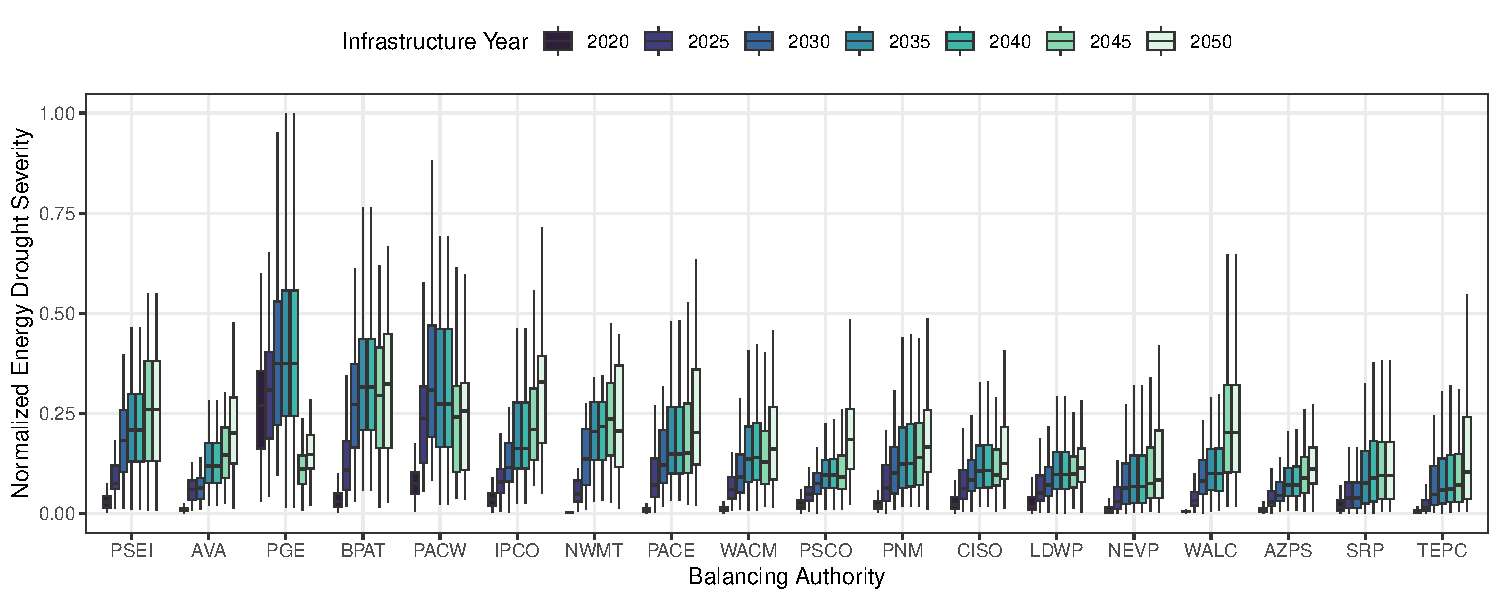
\includegraphics[width=\textwidth]{S1-severity_future_bau_ws_droughts}
    \caption{Energy drought severity (energy deficit below the 10th percentile) for the business-as-usual scenario which involves a fully decarbonized grid by 2050. Climate variability is simulated for each infrastructure year using 40-years of rcp85hotter climate forcing. Severity has been normalized by the maximum value in each BA to allow the data to be compared across BAs and outliers have been removed for visual clarity.}
    \label{fig:severity-bau}
\end{figure}

\begin{figure}
    \centering
    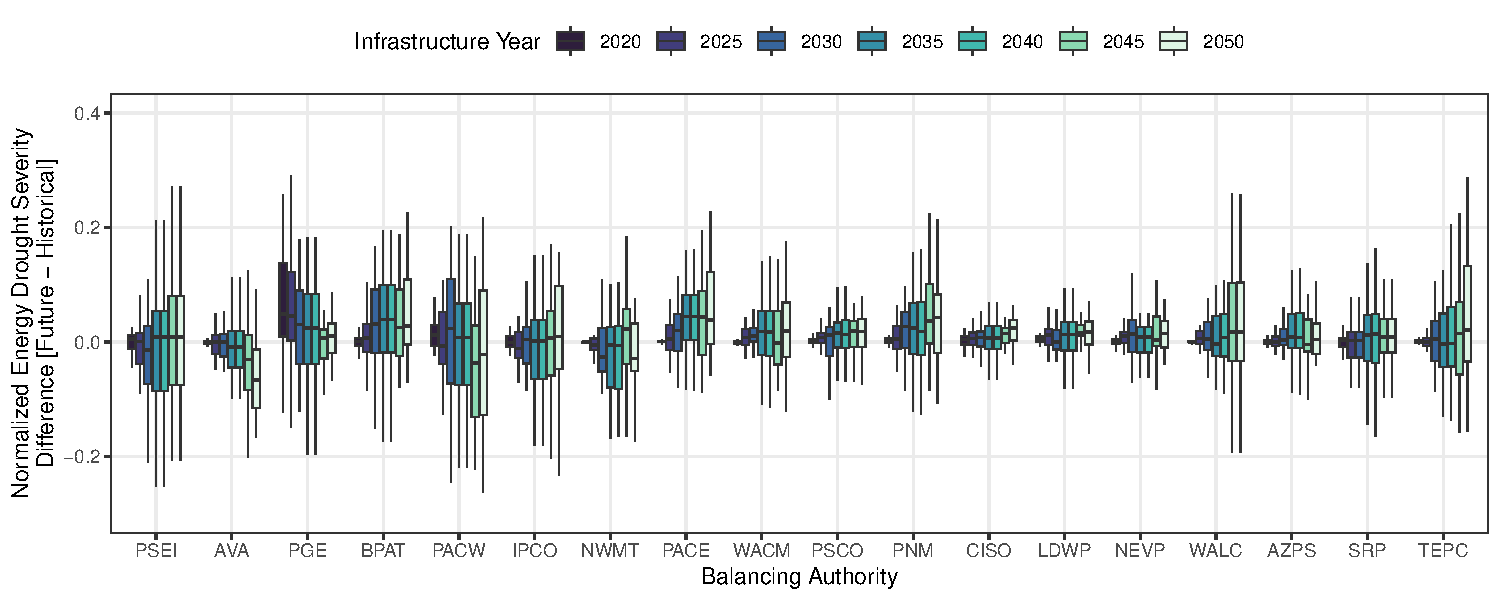
\includegraphics[width=\textwidth]{S2-severity_diff_hist_future_bau_ws_droughts}
    \caption{Difference in average annual normalized energy drought severity between the future and historical periods for the business-as-usual scenario, which involves a fully decarbonized grid by 2050. Severity has been normalized per BA to allow the data to be compared across BAs.}
    \label{fig:severity-diff-bau}
\end{figure}

\begin{figure}
    \centering
    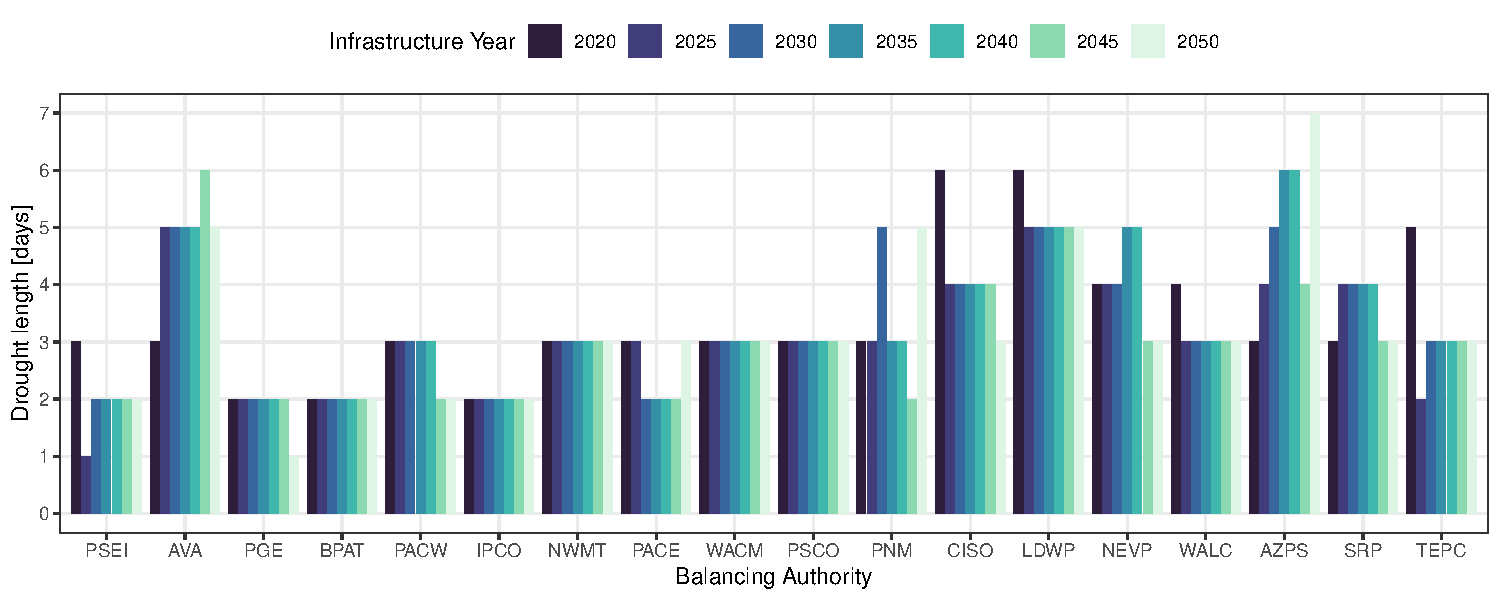
\includegraphics[width=\textwidth]{S3-duration_future_bau_ws_droughts}
    \caption{Energy drought duration for the business-as-usual scenario, which involves a fully decarbonized grid by 2050. Note that the figure does show boxplots, but in most BAs the distribution of drought duration is heavily skewed such that most boxes are collapsed on at the lowest value.}
    \label{fig:duration-bau}
\end{figure}

\begin{figure}
    \centering
    \begin{adjustwidth}{-35mm}{-35mm}
    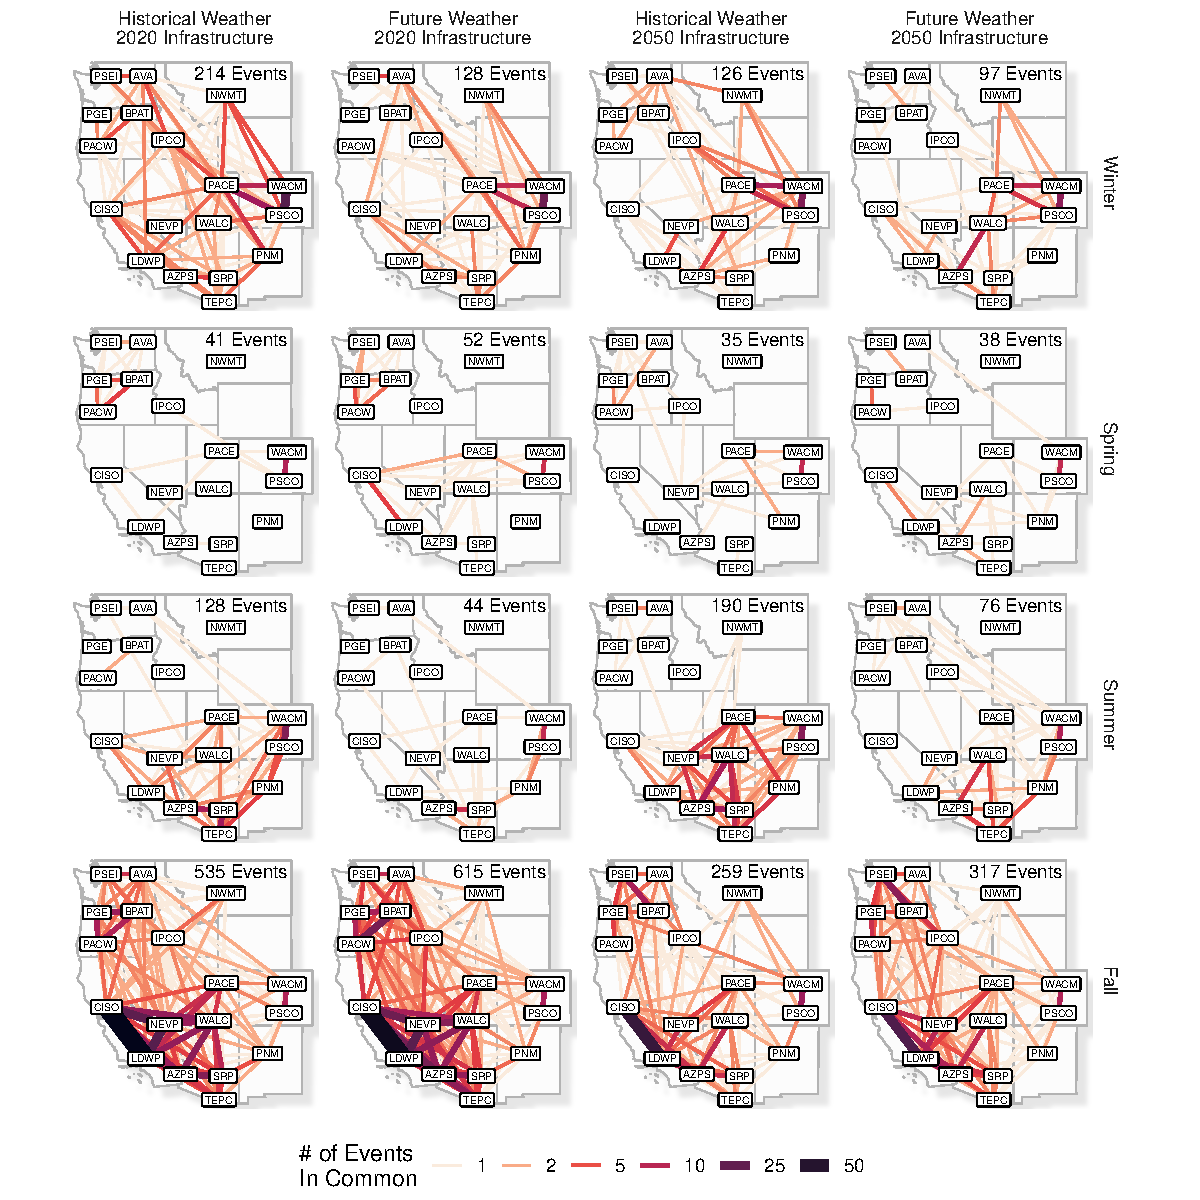
\includegraphics[width=\linewidth]{S4-spatial_connectivity_seasonal_bau_ws_droughts}
    \end{adjustwidth}
    \caption{Seasonal compound energy drought co-occurrence between BAs for the business-as-usual scenario using historical weather with 2020 infrastructure (first column) and future weather with 2020 infrastructure (second column), historical weather with 2050 infrastructure (third column), and future weather with 2050 infrastructure (fourth column). The rows indicate the seasons. A line is drawn between two BAs if at least one energy drought occurred on the same day. The thickness and color of the line represent the number of events in common between a pair of BAs.}
    \label{fig:connectivity-seasonal-bau}
\end{figure}

\begin{figure}
    \centering
    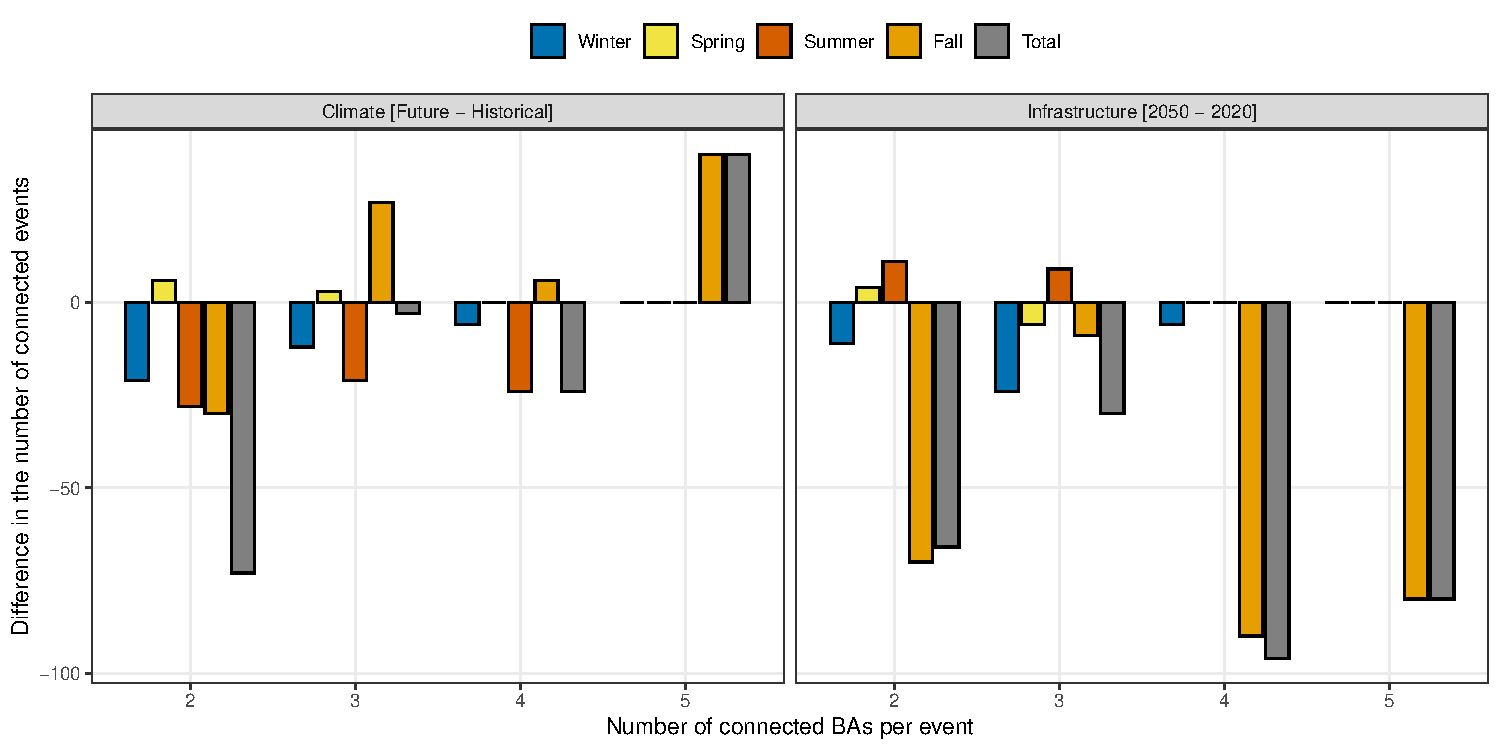
\includegraphics[width=\textwidth]{S5-connected_event_diff_bau_ws_droughts.pdf}
    \caption{The difference between the number of multi-BA compound energy droughts in each season for the business-as-usual scenario. The left panel shows the climate influence by differencing the future weather and historical weather periods using 2050 infrastructure. The right panel shows the infrastructure influence by differencing the 2050 and 2020 infrastructure scenarios both using future weather. Negative values indicate fewer connected events in the future period.}
    \label{fig:connectivity-bau}
\end{figure}


\end{document}




